\chapter[Communication Channels between Colluding Applications]{Analysis of the Communication between Colluding Applications on
  Modern Smartphones}
\label{chap:sp_appcollusion}

\newcommand{\noinch}[1]{\noindent \emph{#1:}}

\section{Introduction}

Modern smartphone operating systems allow users to install third-party
applications directly from on-line \emph{application markets}. Given
the large number of applications and different independent developers,
every application cannot be trusted to behave according to its
declared purpose. Certain types of malicious behaviors can be detected
by inspection and testing while others cannot; malicious applications
therefore find their way into the application
markets~\cite{Stajano_inglorious_installers,Android_malware_Oberhide,Mobile_harder_than_fixed,App_centric_android_security}.

To limit the potential impact of malicious applications, mobile phone
operating systems (e.g., Android OS~\cite{os-android}, Windows Phone~\cite{os-wp7}) implement a
permission-based security model (also called a \emph{capability
  model}) that restricts the operations that each application can
perform. This model explicitly gives permissions to applications in
order for them to execute their required operations. Recent work by
Schlegel et al.~\cite{soundcomber-ndss} introduces smartphone malware
that makes use of application collusion over a limited number of
communication channels to overcome the security mechanisms put in
place by the implemented permission-based model. By establishing
communication over a covert or overt channel, applications are allowed
to execute operations which the system, based on their declared
permissions, should prohibit.

It is important to stress that application collusion attacks on
permission-based models are not a result of a software vulnerability
and are not related to a particular implementation. Instead, they are
a consequence of the basic assumption on which the permission-based
model relies: applications can be independently restricted in
accessing resources and then safely composed on a single
platform. Collusion attacks show that this assumption is incorrect and
can be exploited to circumvent the permission-based
model. Furthermore, in current systems, users are not made aware of
possible implications of application collusion attacks---quite the
contrary---users are implicitly lead to believe that by approving the
installation of individual applications independently, they can limit
the damage that an application can cause.

Although the existence of overt and covert channels and thus the
feasibility of application collusion on any platform might not be
surprising, the implications of collusion are very damaging on mobile
platforms: these platforms are designed for personal use, generally
store personal information and facilitate the installation of multiple
third-party applications. Furthermore, existing security products
(e.g., Lookout Privacy Advisor~\cite{lookout_privacy_advisor}) analyze
and report application permissions independently for each individual
application. Since they do not consider application collusion, these
products do not correctly reflect the collective privacy implications
of the applications that the users install.

In this work, we demonstrate the existence of a number of overt and
covert channels by implementing them on an Android platform. We then
evaluate the severity of the threats posed by application collusion
attacks by measuring the throughput and stability of each channel. Our
results show that different covert channels, which are generally hard
to detect or prevent, can reach throughputs ranging from 3.70 bps up to
roughly 3.27 kbps on the Nexus One and from 0.47 bps up to 4.22 kbps
on the Samsung Galaxy S, thus posing a serious threat to privacy on
modern smartphones.

While it has been shown that overt channels on mobile smartphones may
be detected and restricted by using taint analysis~\cite{taintdroid},
policy enforcement~\cite{TUD-CS-2011-0127,newxmandroid}, better
sandboxing and by reducing access to some APIs, we show that these
approaches fail to detect most covert channels. This is consistent
with research carried out in the 1970's where it has been shown that
covert channels in computer systems are hard to
prevent~\cite{Denning:1979:DS:356778.356782,Lipner:comment_on_confinment}. To
evaluate the effectiveness of contemporary tools, we tested both
TaintDroid~\cite{taintdroid} and XManDroid~\cite{newxmandroid} and
confirmed that they do not detect all channels and therefore fail to
fully prevent application collusion. This shows that application
collusion attacks remain a real threat on modern smartphone
platforms. Finally, we propose ways of preventing or limiting some of
these channels.

In summary, the contributions of this chapter are the following. (1) We
demonstrate the practicality of application collusion attacks by
implementing several communication channels on the Android
platform. (2) We measure and report the throughput of implemented
communication channels highlighting the extent of the threat posed by
such attacks. (3) We confirm that two recently proposed architecture
modifications and tools that deal with overt and covert channels
discovery, TaintDroid~\cite{taintdroid} and
XManDroid~\cite{newxmandroid}, still fail at detecting several of the
implemented channels. (4) We propose countermeasures that, if not
eliminate, limit the capacity of selected communication channels
between the applications.

\section{Problem Statement}
\label{sec:sp_appcollusion_prob-stat}

The goal of this work is to understand the threat posed by colluding
applications on modern smartphones. In particular we investigate the
feasibility and the practicality of multiple communication channels in
terms of throughput, bit-error rate and required
synchronization. Figure~\ref{fig:sp_appcollusion_simple-channel} illustrates an
example channel between two applications. On the left, the
\emph{ContactsManager} application has access to private data on the
device but not to the network (later in the work referred to as the
\emph{source} application), on the right, the \emph{Weather}
application having access to the network but no direct access to the
private data (later in the work referred to as the \emph{sink}
application). The two applications can create a stealthy communication
channel to share data. Figure~\ref{fig:sp_appcollusion_browserchannel} illustrates an
interesting covert channel that can be created between an application
and the Browser which does not require any extra application to be
installed on the device. We will describe this channel in more detail
in Section~\ref{sec:sp_appcollusion_browserchannel}.

\begin{figure}[!ht]
	\centering
	\subfigure[]{
	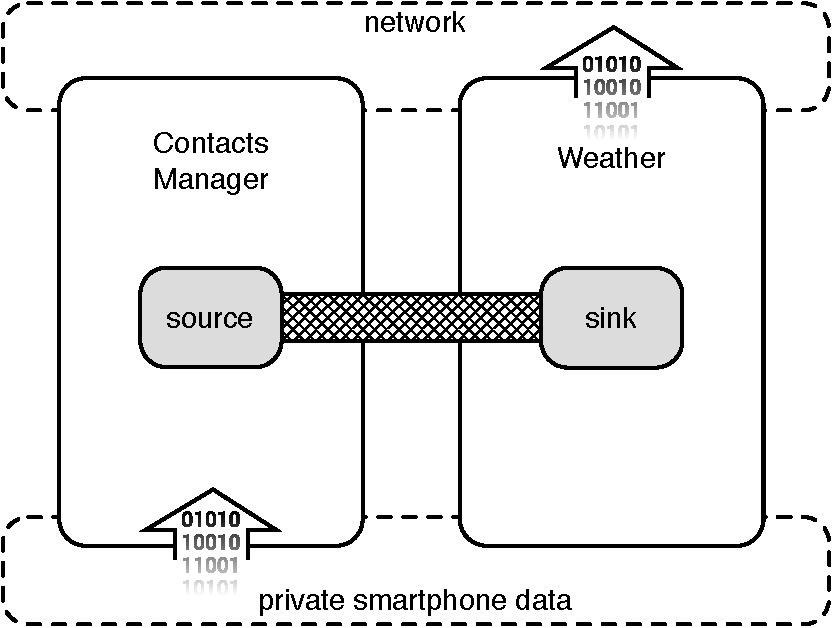
\includegraphics[width = .47\textwidth]{figures/securingphone/channels_source_sink.pdf}
	\label{fig:sp_appcollusion_simple-channel}
	}
	\subfigure[]{
	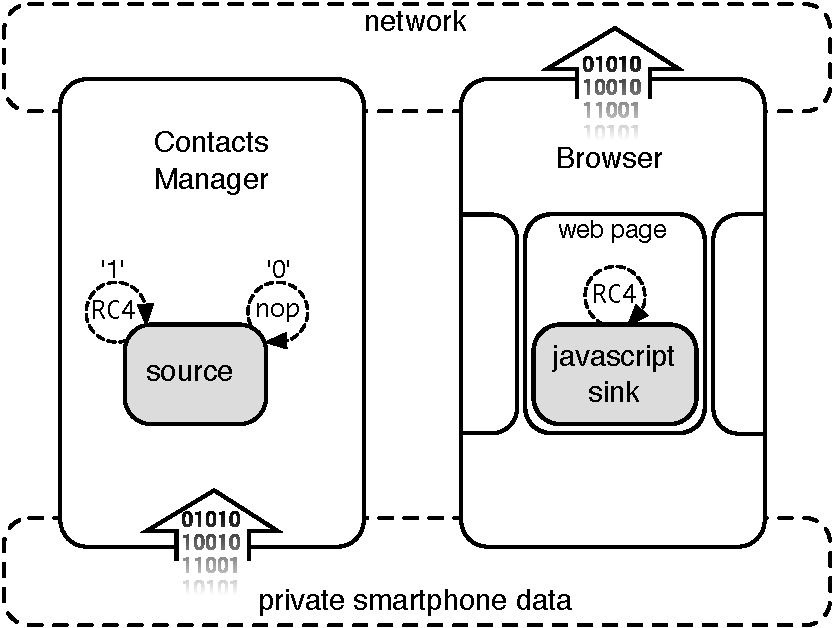
\includegraphics[width = .47\textwidth]{figures/securingphone/channels_browser_channel.pdf}
	\label{fig:sp_appcollusion_browserchannel}
	}
	\caption[Examples of overt and covert channels]{On the left, Figure (a) shows a generic example of collusion
between the \emph{ContactsManager} and the \emph{Weather} applications through a stealthy (overt) communication channel. On the right, Figure (b) shows a (covert) timing channel between an application and the browser working through the use of dummy RC4 operations.}
	\label{fig:sp_appcollusion_example-channel}
\end{figure}

\subsection{Channels Classification}
\begin{table*}[t!]
  \centering
  \scalebox{.9}{%
    \begin{tabular}{|p{.4\textwidth}|rl|rl|} \hline
      \textbf{Overt Channel} & \multicolumn{4}{|c|}{\textbf{Throughput (kbps)}}
      \\ \hline
      & \multicolumn{2}{|c|}{Nexus One} & \multicolumn{2}{|c|}{Samsung
        Galaxy S} \\ \hline \hline
      UNIX Socket Communication & 340.45 & ($\pm$ 154.02) & 34.78 &
      ($\pm$ 11.39) \\ \hline
      Internal Storage & 292.03 & ($\pm$ 50.06) & 32.60 & ($\pm$ 8.47)
      \\ \hline
      Shared Preferences & 75.81 & ($\pm$ 6.83) & 31.00 & ($\pm$ 2.75)
      \\ \hline
      Broadcast Intents & 40.58 & ($\pm$ 8.41) & 26.74 & ($\pm$ 4.88)
      \\ \hline
      External Storage $\dagger$ & 11.55 & ($\pm$ 1.10) & 6.12 &
      ($\pm$ 3.95) \\ \hline 
      \textbf{System Log} $\ddagger$ & 2.94 & ($\pm$ 0.03) & 2.14 &
      ($\pm$ 0.11) \\ \hline

      \multicolumn{5}{l}{\textbf{$\dagger$}
        Requires extra \texttt{WRITE\_EXTERNAL\_STORAGE} permission.}\\
      \multicolumn{5}{l}{\textbf{$\ddagger$}
        Requires extra \texttt{READ\_LOGS} permission.} \\
      %\multicolumn{5}{l}{} % just for spacing
    \end{tabular}}
  \caption[List of our implemented \emph{overt} channels in the
    Android OS with corresponding throughputs]{List of our implemented \emph{overt} channels in the
    Android OS with corresponding throughputs (with the 95\% confidence
    intervals in parenthesis). The displayed values are averaged over 10 runs
    for both the Nexus One and the Samsung Galaxy S. The ``System Log'' is a new channel that we engineered and for which
    we did not find references in the open literature.}
  \label{tab:sp_appcollusion_overt-channels}
\end{table*}

We classify communication channels based on their implementation on
current smartphone architectures as follows:

\begin{itemize}
\item \textbf{Application.} This is the level of the API that an
  operating system provides to the developers (e.g., Android's Java
  API, Windows Phone 7 C~\# / Silverlight APIs, iOS's Objective-C
  API). Access and usage of these communication channels may be easily
  controlled. We consider these channels as \emph{high}-level.
\item \textbf{OS.} This is the level of the operating system that is
  exposed through native calls that exploit information present in the
  operating system. We believe that at this level some channels are
  impossible to close, others, if closed, could hamper backward
  compatibility severely.
\item \textbf{Hardware.} This is the level that is exposed through
  exploiting hardware functionalities of the smartphone. It is highly
  dependent on individual hardware specifications of smartphone
  models. These communication channels cannot be closed without severe
  performance degradation of the system. We consider these channels as
  \emph{low}-level.
\end{itemize}

Different levels usually also imply different throughput and
stealth. In particular, we notice that throughput is usually directly
proportional to the level, with higher throughput associated to
\emph{high}-level communication channels. Stealth (i.e., the
difficulty to detect a communication channel), on the other hand, is
usually inversely proportional to the level, with stealthier channels
associated to \emph{low}-level communication channels.

% In some cases low-level channels can achieve better results due to
% implementation details that could be exploited to improve the
% performance of a communication channel.

\section{Overt and Covert Channels in Android}
\label{sec:sp_appcollusion_case-study}
We explore possible covert and overt channels on Android
smartphones. We analyzed some known channels and identified a number
of new channels specific to smartphones not yet presented in the
literature.

To analyze overt and covert channels, we implemented a framework to
measure the throughput, the bit error rates and the synchronization
times for each implemented communication channel. The results of our
study are presented in
Tables~\ref{tab:sp_appcollusion_overt-channels}~and~\ref{tab:sp_appcollusion_covert-channels}.

The values shown in both tables are averaged over 10 independent runs
for each implemented channel executing on a Nexus One or a Samsung
Galaxy S smartphone. During the tests the phone was running on battery
power and not charging. Each time the \emph{source} application tries
to send 4, 8 and 135 byte (to mimic the transfer of contact
information as explained in Section~\ref{sec:sp_appcollusion_resultsanalysis})
messages to the \emph{sink} that, if the channel is open, would record
them successfully. For each covert channel that requires tight
synchronization between the \emph{source} and the \emph{sink}
application (i.e., timing channels), we implement a synchronization
protocol and run it before starting to send data. In general the
synchronization protocol is used to estimate the noise present in the
system when the applications want to share data and to correctly start
the measurements to exchange data at the same time. Such a protocol is
implemented on top of the covert channel (i.e., using the same
mechanism) and allows us to reach higher accuracy. A covert channel's
accuracy is measured in bit error rate, with perfectly accurate
channels reaching 0\% bit error rate during transmission. While
synchronization time values are reported in
Table~\ref{tab:sp_appcollusion_covert-channels} for completeness, we believe that they
can be further optimized to yield overall slightly faster
communication channels.

\subsection{Overt Channels}

We now briefly describe the implementation of overt channels to give
an intuition of how they work.

\noinch{Shared Preferences (Application)} the \emph{sink} application
uses an API to create an Android preference XML file that is
world-readable and world-writable. The \emph{source} application
writes ASCII data to it and the \emph{sink} reads it. This channel
does not require any synchronization to operate as the two
applications do not need to be run simultaneously.

\noinch{Internal Storage (Application)} the \emph{source} application
writes a world-readable file to the internal storage, the \emph{sink}
application reads its contents. Similarly the \emph{External Storage}
simply uses a file on the external storage. For the external channel
to work, the \emph{source} application requires an extra permission:
\texttt{WRITE\_EXTERNAL\_STORAGE}. Again, similar to the \emph{Shared
  Preferences} communication channel, these channels do not require
synchronization between the applications.

\noinch{Broadcast Intents (Application)} the \emph{source} application
communicates by adding private data as extra payload to a broadcast
message sent to the system. Broadcast intents are a particular type of
messages that are used in the Android OS to enable one form of
communication between applications. The operating system, upon
receiving such a message with its payload, broadcasts it to all the
applications that requested to be notified when such a message is
received (i.e., by registering themselves for a particular ID that is
used to identify the message). The \emph{sink} application registers
itself with the system and receives the message sent by the
\emph{source}. While both applications need to be running at the same
time, no synchronization is required in order for the channel to work.

\noinch{System Log (Application)} the \emph{source} writes a
specially-crafted message to the system log that the \emph{sink} then
reads to extract the information. The extra \texttt{READ\_LOGS}
permission is required by the \emph{sink} application in order to be
able to read the system logs. Messages longer than 4000 characters
must be split and binary data must be encoded, because data is
otherwise lost when inserted into the log. Given that the log has a
finite number of entries that are held at any time, the \emph{sink}
application must be activated before the message sent by the
\emph{source} is deleted. Alternatively, the \emph{source} could
repeatedly insert the message at time intervals to increase the chance
that the \emph{sink} receives it. Potentially the channel can be
rendered stealthy by filling the log with seemingly meaningful logging
data after the communication takes place.

\noinch{UNIX Socket Communication (OS)} the \emph{source} sends the
data through a UNIX socket that the \emph{sink} application opened.
For this channel to work correctly, both applications must be
simultaneously active.

\subsection{Covert Channels}

We now describe the covert channels that we implemented and measured.
As the storage of these channels is not persistent, all these channels
are synchronous. This means that before starting to exchange data over
the channel a synchronization protocol between the \emph{source} and
the \emph{sink} must be run in order to achieve better accuracy during
the data-exchange phase. For channels where accuracy is not
specifically stated, our implementation reached perfect accuracy.

\noinch{Single and Multiple Settings (Application)} the \emph{source}
modifies a general setting on the phone and the \emph{sink} reads it
as described in~\cite{soundcomber-ndss}. Multiple settings can be
changed at the same time to achieve higher throughput. Most settings
in Android can be changed and read without requesting any
permissions. This particular covert channel can be closed by disabling
or requiring extra permissions in order to change particular settings.

\noinch{Type of Intents (Application)} the \emph{source} sends a
broadcast message (similar to the \emph{Broadcast Intents} overt
channel) to the \emph{sink} and encodes the data to be transmitted
into the type of the intent (i.e., flags, action, particular extra
data), rather than directly exchanging the data as the extra payload
of the message. In contrast to the similar overt channel that uses
\emph{Broadcast Intents}, this covert channel is not detectable by
tainting mechanisms or similar solutions. The \emph{sink} application
still needs to register with the system in order to receive the
intents.

\noinch{Automatic Intents (Application/OS)} the \emph{source} modifies
particular settings (i.e., the vibration
setting~\cite{soundcomber-ndss}) that trigger automatic broadcasts by
the system to all applications that registered to be notified when
such a change happens. The \emph{sink} receives the messages and
infers the data depending on the contents of the received
broadcasts. For instance, changing the vibration setting of the phone
triggers a broadcast which contains 1-bit of information (vibration on
equals to 1, vibration off equals to 0).

\noinch{Threads Enumeration (OS)} the \emph{source} spawns a number of
threads and the \emph{sink} reads how many threads are currently
active for the source application by looking into the \texttt{/proc}
directory of \emph{source}. This particular covert channel can be
closed by controlling application access to the \texttt{/proc}
filesystem or by mediating the access through a system service.

\begin{landscape}
\begin{table}[!ht]
  \centering
  \scalebox{.8}{%
    \begin{tabular}{|l|rl|rl|rl|rl|} \hline
      \textbf{Covert Channel} &
      \multicolumn{4}{|c|}{\textbf{Throughput (bps)}} &
      \multicolumn{4}{|c|}{\textbf{Synchronization (ms)}} \\ \hline
      & \multicolumn{2}{|c|}{Nexus One} & \multicolumn{2}{|c|}{Samsung
        Galaxy S} & \multicolumn{2}{|c|}{Nexus One} &
      \multicolumn{2}{|c|}{Samsung Galaxy S} \\ \hline \hline

      
      \textbf{Type of Intents} & 3350.85 & ($\pm$ 134.11) & 4324.13 &
      ($\pm$ 555.32) & 716.8 & ($\pm$ 168.2) & 473.0 & ($\pm$ 249.0) \\ \hline
      \textbf{UNIX Socket Discovery} & 2610.92 & ($\pm$ 305.25) &
      1647.78 & ($\pm$ 170.70) & 5.2 & ($\pm$ 0.8) & 13.9 & ($\pm$ 2.2) \\ \hline
      Multiple Settings & 239.76 & ($\pm$ 9.41) & 284.91 & ($\pm$
      1.90) & 314.9 & ($\pm$ 21.8) & 302.1 & ($\pm$ 11.0) \\ \hline
      \textbf{Threads Enumeration} & 157.73 & ($\pm$ 0.97) & 139.39 &
      ($\pm$ 7.40) & 71.6 & ($\pm$ 7.1) & 110.1 & ($\pm$ 8.8) \\ \hline
      Automatic Intents~\cite{soundcomber-ndss} & 51.38
      & ($\pm$ 0.41) & 90.67 & ($\pm$ 0.39) & 1083.2 & ($\pm$ 75.1) &
      435.1 & ($\pm$ 180.8) \\ \hline
      Single Settings~\cite{soundcomber-ndss} & 46.88 & ($\pm$ 0.31) &
      65.89 & ($\pm$ 0.73) & 267.5 & ($\pm$ 3.2) & 273.4 & ($\pm$ 11.9)
      \\ \hline
      Free Space on Filesystem & 13.07 & ($\pm$ 0.00) & 9.80 & ($\pm$
      0.00) & 1038.2 & ($\pm$ 5.1) & 1442.7 & ($\pm$ 15.6) \\ \hline
      \textbf{Reading \texttt{/proc/stat}} & 7.82 & ($\pm$ 0.00) &
      3.26 & ($\pm$ 0.00) & 6923.4 & ($\pm$ 8.1) & 16669.2 & ($\pm$
      48.7) \\ \hline
      \textbf{Processor Frequency} & 4.88 & ($\pm$ 0.00) & 0.47 &
      ($\pm$ 0.09) & 8203.9 & ($\pm$ 7.2) & 78866.1 & ($\pm$ 9156.8)
      \\ \hline
      Timing Channel & 3.70 & ($\pm$ 0.00) & 3.69 & ($\pm$ 0.01) &
      10286.8 & ($\pm$ 16.1) & 68057.6 & ($\pm$ 105259.4) \\ \hline

      \multicolumn{9}{l}{} % just for spacing
    \end{tabular}}

  \caption[List of implemented \emph{covert} channels in the
    Android OS with their corresponding throughput]{List of implemented \emph{covert} channels in the
    Android OS with their corresponding throughput (95\% confidence
    intervals are shown in parenthesis). The displayed values are averaged over 10 runs
    for both the Nexus One and the Samsung Galaxy S. Channels listed
    in \textbf{bold} are new channels that we engineered and for which
    we did not find references in the open literature. In the
    synchronization column we present the time required to run the
    synchronization protocol before starting to transmit data through
    the channel.}
  \label{tab:sp_appcollusion_covert-channels}
\end{table}
\end{landscape}

\noinch{UNIX Socket Discovery (OS)} the \emph{source} uses two
sockets, a synchronization socket and a communication socket. The
\emph{sink} checks if the \emph{source} communication socket's state
is open, and infers the transferred bit. The synchronization socket is
open if the communication socket can be checked.

\noinch{Free Space on Filesystem (OS)} the \emph{source} application
writes or deletes data on the disk to encode the information for the
\emph{sink}. The channel throughput depends on the noise in the
system; for example the sink application could infer a larger amount
of information depending on how many free blocks are available. The
data presented in Table~\ref{tab:sp_appcollusion_covert-channels} was generated by
having the \emph{source} allocate three blocks to encode a `1' and
clearing three blocks to encode a `0'. The \emph{sink} checked the
available blocks in the system at predefined time intervals (75ms for
the Nexus One and 100ms for the Galaxy S). The current implementation
yields bit-errors percentages between 0.01\% (Nexus One) and 0.03\%
(Samsung Galaxy S). A possible solution for preventing this channel is
to enforce a quota on the available space for each application (that
could potentially vary depending on the number of applications on the
system) and report the free blocks remaining of each quota rather than
the free blocks in the overall system.

\begin{figure}[!ht]
  \centering
  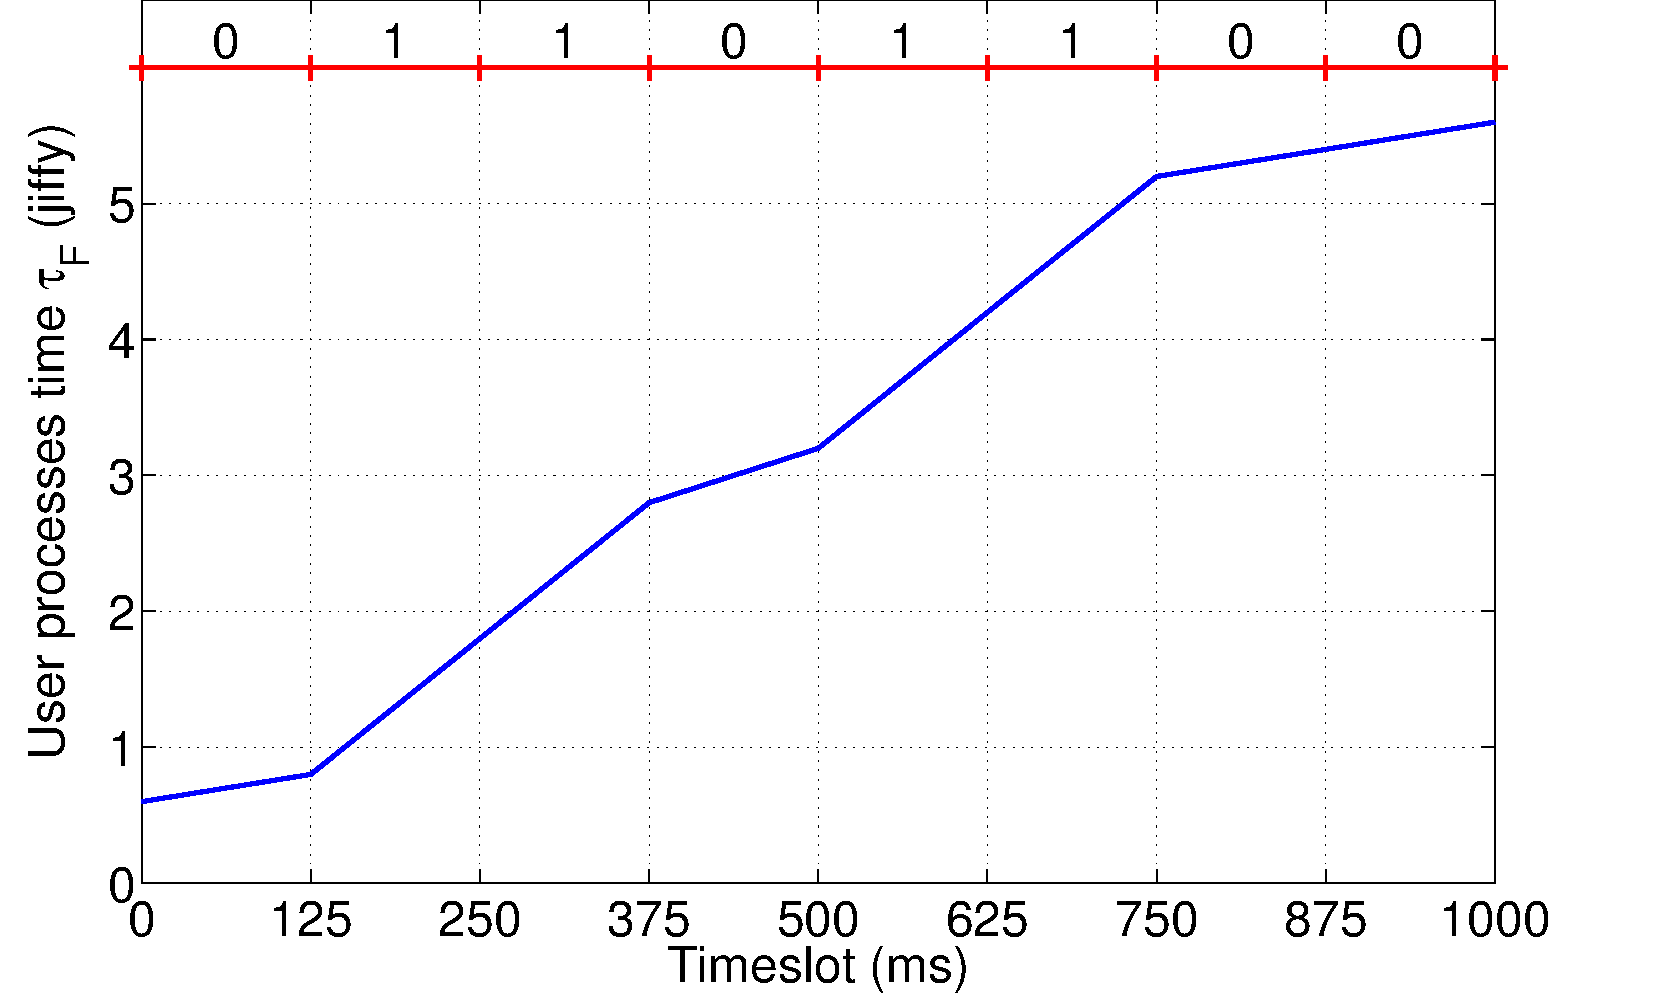
\includegraphics[width=.8\linewidth]{figures/securingphone/channels_p1}
  \caption[Schematic rise of the value $\tau_F$ over time]{Exemplification schematic rise
  of the value $\tau_F$ (number of jiffies spent for every user process) over time when
  sending the bits written on the top.}
  \label{fig:sp_appcollusion_procstata}
\end{figure}

\noindent \emph{Reading} \texttt{/proc/stat} \emph{(OS):} the
\emph{source} application performs some computations, while the
\emph{sink} monitors the processor usage statistics. These are
available in the \texttt{/proc/stat} virtual file where the Linux
kernel provides information about the current system load (as the
number of jiffies used for all user processes). A schematic
representation of how the values ($\tau_F$) read in
\texttt{/proc/stat} change depending on the bit that the \emph{source}
wants to send is presented in Figure~\ref{fig:sp_appcollusion_procstata}. The overall
idea is that sending a `1' causes, in the values read, a steeper slope
than sending a `0'. Figure~\ref{fig:sp_appcollusion_procstatb} presents the trade-off
between throughput and accuracy of this channel. Other channels behave
similarly to this one, with higher throughput resulting into lower
accuracy. The current implementation yields bit-error percentages
between 0\% (Samsung Galaxy S) and 0.10\% (Nexus One). Similarly to
the \emph{Threads Enumeration} covert channel, this channel could be
closed by preventing read access to the \texttt{/proc} filesystem.

\begin{figure}[!ht]
	\centering
	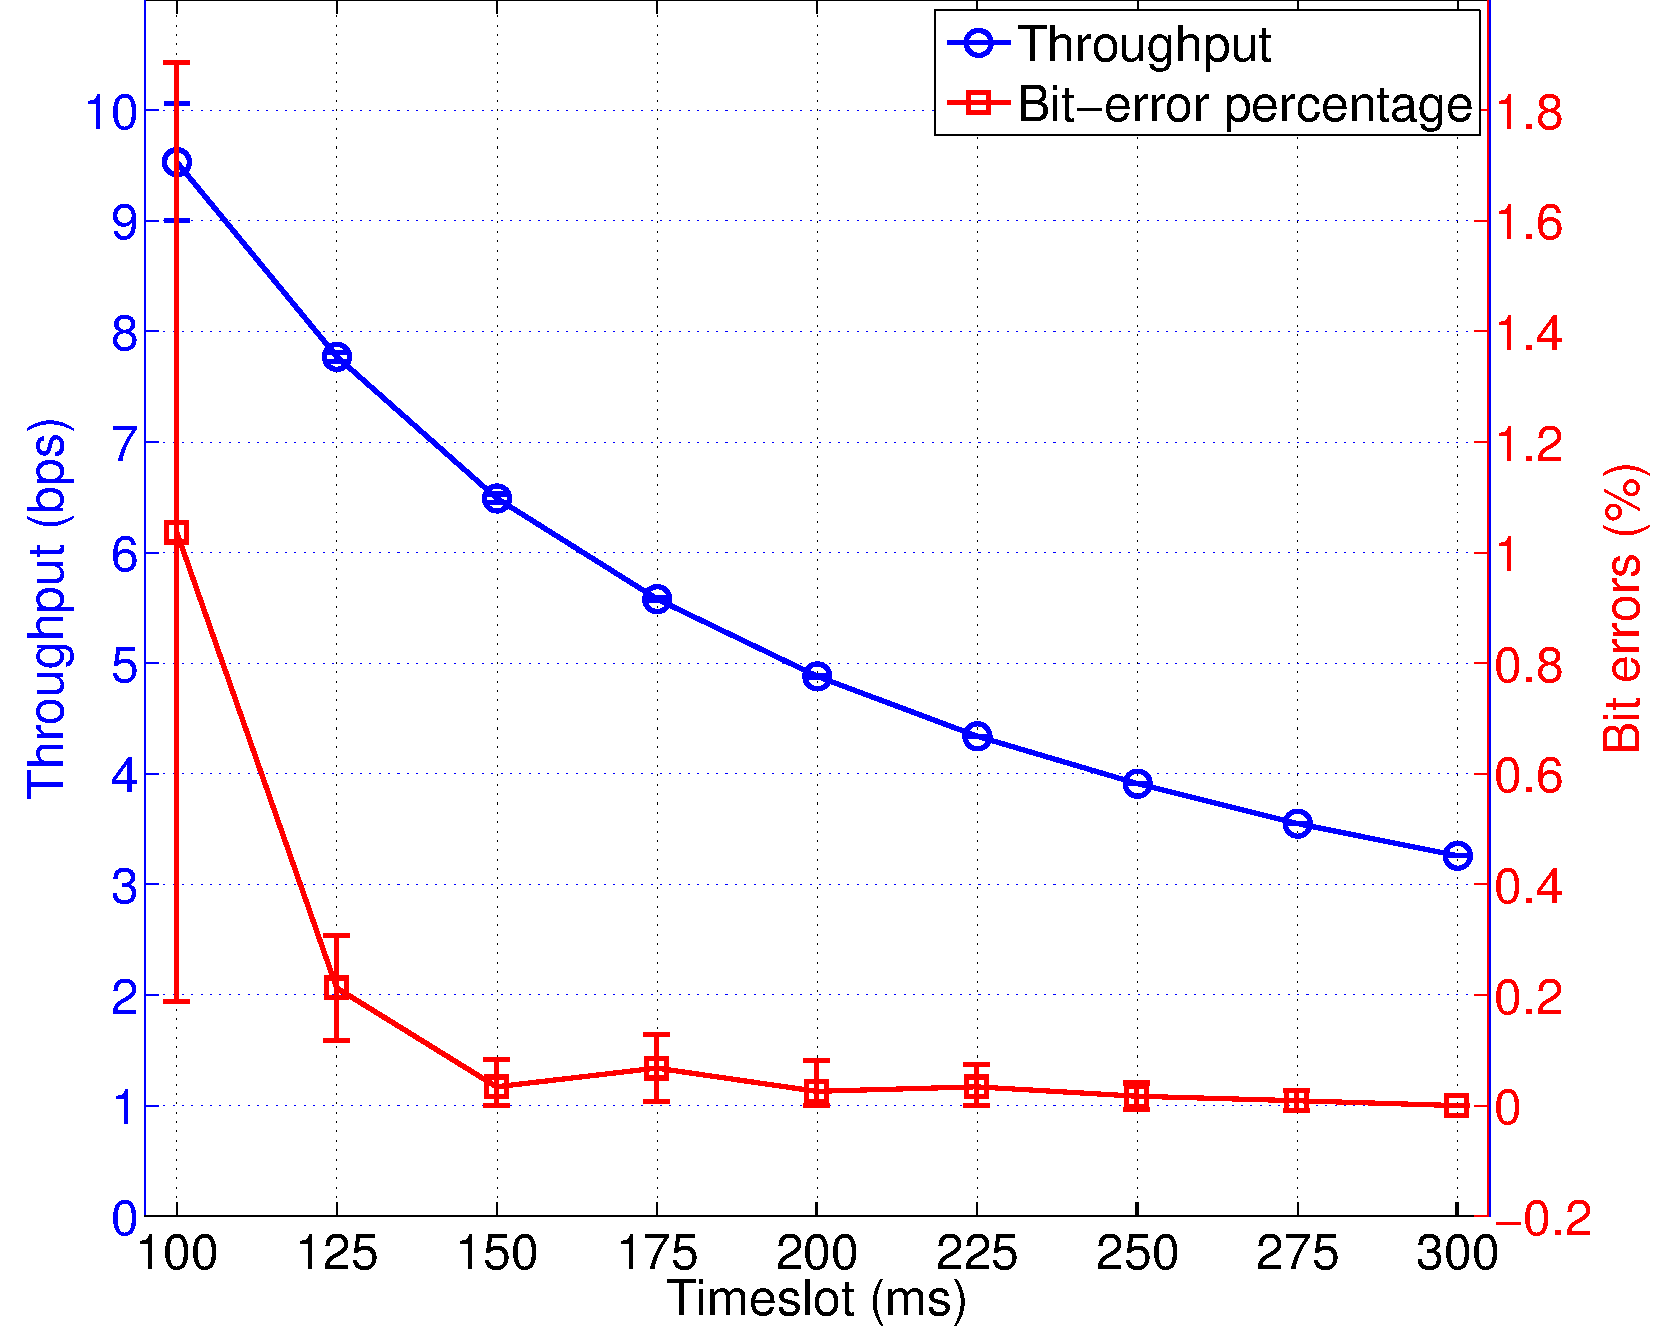
\includegraphics[width=.8\linewidth]{figures/securingphone/channels_p2}
	\caption[Trade-off between throughput and accuracy]{The graph shows the trade-off
between throughput and accuracy (measured in bit errors) for the \texttt{/proc/stat}
channel. Values are averaged over 5 independent runs.}
	\label{fig:sp_appcollusion_procstatb}
\end{figure}

\noinch{Timing Channel (Hardware)} the data transmission between the
source and the sink is performed by varying the load on the
system. The \emph{source} runs CPU-intensive tasks to send the bit
`1', on the other hand it does not perform any CPU-intensive operation
to send the bit `0'. The \emph{sink} continuously runs
computation-intensive operations and records the time required to
complete them. The \emph{sink} uses this time to infer the presence of
computation by the \emph{source} thus inferring the transmitted
bit. For reliable differentiation of bits based on the time, an
initial \emph{learning period} is used to benchmark the system
behavior. Finally, to eliminate the noise in the system, we use a
majority vote (out of five measurements) at the \emph{sink} to decide
the value of a particular bit depending on a threshold value updated
with a moving average. In our implementation, the time difference
between transmitting a `1' and a `0' is approximately 6 ms in the case
of the Nexus One. The current implementation yields bit-errors
percentages between 0.10\% (Nexus One) and 0.05\% (Samsung Galaxy S).

To better visualize the majority vote mechanism used in our
implementation, in Figure~\ref{fig:sp_appcollusion_timing} we present an example
trace of the measurements taken at the \emph{sink}. The blue dots
represent measurements done while the \emph{source} was sending a
`1', the green crosses while it was sending a `0'. 5400 measurements
were performed to send the test message of 135 bytes (1080 bits) as
it is shown in the figure.

\begin{figure}[!t]
  \centering
  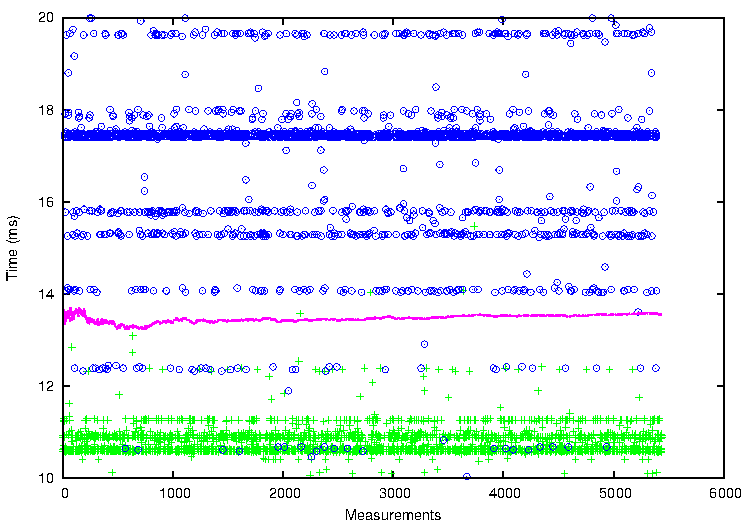
\includegraphics[scale=.65]{figures/securingphone/channels_timingpaper_weight}
  \caption[Measurements taken by the \emph{sink} application to infer
    information sent over a Timing Channel]{Measurements taken by the \emph{sink} application to infer
    information sent over a Timing Channel. The blue dots show
    measurements while the \emph{source} is sending a `1', green
    crosses while it is sending a `0'. 5400 measurements are needed to
    receive a 135-byte message (5 measurements are used to assign a
    value to a bit through a majority-vote mechanism). The red line
    shows a moving average used as a threshold value.}
  \label{fig:sp_appcollusion_timing}
\end{figure}

\noinch{Processor Frequency (Hardware)} this channel is an improvement
over the basic \emph{Timing Channel}; in this particular instance we
take into account Dynamic Frequency Scaling (used on the smartphones
that we tested) to improve the throughput and reduce the
synchronization time (for the Nexus One). While the \emph{source}
behavior remains the same as in the case of the \emph{Timing Channel},
the \emph{sink} instead monitors the trend of the processor frequency
by repeatedly querying it from the system and thereby decodes the
current bit. Afterwards the \emph{source} waits a fixed amount of time
to allow the CPU to ``slow down'' again before the next bit
transmission is started. The current implementation yields bit error
percentages between 0.14\% (Nexus One) and 4.67\% (Samsung Galaxy S).

\subsection{Communication Channel With External Agents}
\label{sec:sp_appcollusion_browserchannel}

We extend the concept of colluding applications and consider the
scenario in which there is only one application installed on the
system that has access to private data and wants to disclose it to a
third-party web service without requesting the permissions to connect
to the network. Furthermore, we want to ensure the successful
transmission of the private data through a channel that is hard to
detect. Here, the colluding \emph{sink} application resides on a web
page executing intensive JavaScript operations, that is opened within
the system browser. The phone will show the page on the screen,
therefore, to decrease detection by the user, the operation can be
carried out when the phone screen is off (for example, during night
time). To reach the \emph{sink}, the \emph{source} application uses a
covert timing channel similar to the \emph{Processor Frequency} covert
channel. However the \emph{sink} cannot directly query the processor
frequency, as it is inside the JavaScript sandbox. Such channel is
visualized in Figure~\ref{fig:sp_appcollusion_browserchannel}.

We have implemented and tested this proposed covert channel as
follows: depending on the current bit to transfer, the \emph{source}
either tries to increase the processor frequency or sleeps. Afterwards
the \emph{sink} measures how many dummy RC4 operations it can perform
in a fixed time period, thereby getting the processor frequency and
the transmitted bit. The possibility to use the browser to send
private data has been described in~\cite{permissions-browser} but
their proposed method is easily detected by flow-tracking techniques
(such as TaintDroid). Our proposed covert channel---while having a low
throughput of roughly 1.29bps on the Nexus One---is also much harder
to detect and cannot be detected by today's tools.

\subsection{Results of the Analysis}
\label{sec:sp_appcollusion_resultsanalysis}
The experiment results reported in Tables~\ref{tab:sp_appcollusion_overt-channels}
and~\ref{tab:sp_appcollusion_covert-channels} indicate that the attacker's choice of
one channel over another, depends on the nature and size of data that
needs to be transmitted between applications. For example GPS
coordinates usually consist of two floating point numbers (represented
by 32 bits of data), in contrast contacts, for example, might have a
varying number of characters: in order to simulate a few full names
and corresponding phone numbers we transmit 135 bytes of information.

Given a rough estimate of the size of the data that can be shared
between applications, we conclude that even the covert channels with
low throughput, such as the \emph{Timing} or the \emph{Processor
  Frequency} channels (respectively at around 3.70 and 4.88 bps)
enable the sharing of reasonable amounts of data on the
smartphone. For example, exchanging GPS coordinates requires roughly
19.4 or 14.8 seconds respectively; sharing 135 byte contacts requires
roughly 304.9 or 231.1 seconds respectively. Covert channels with
higher throughput, such as the \emph{Type of Intents} or \emph{UNIX
  Socket Discovery}, reaching up to 4324.13 and 2610.92 bps, enable
the exchange of GPS coordinates or contact information in less than a
second.

Another interesting result of the analysis is that most channels, when
tested on the more powerful Samsung Galaxy S, did not perform better
than on the Nexus One. For CPU-bound channels these results come from
the fact that Samsung ships the device with a larger number of active
services which influence the different channels. For channels based on
Processor Frequency it is based on the fact that there is a different
frequency governor. For IO-bound channels these results come from the
fact that the Samsung device uses a Samsung-developed file system
rather then the standard YAFFS2 used on the Nexus One.

Overall, the results show that application collusion attacks, through
the usage of different communication channels depending on the amount
of data that needs to be transmitted, are a realistic attack and
therefore a serious threat.

\section{Analysis of Existing Tools}
\label{sec:sp_appcollusion_analysis-existing-solutions}
In this Section we test two recently proposed tools that try to solve
the information leakage on modern smartphones, in particular
TaintDroid~\cite{taintdroid} and XManDroid~\cite{newxmandroid}. We use
the Nexus One as the test phone where we successfully install both
tools and report the findings.

\subsection{TaintDroid}

TaintDroid~\cite{taintdroid} tries to track information flows within
an application and between applications; it is implemented as a
modification of the Android operating system. Using dynamic
taint-tracking, the modified OS follows the information flow of tagged
data, that is, data which is generated from sources of private
information, including the user contacts and the GPS location.

Inside the Dalvik VM, TaintDroid employs variable tracking and
propagates taint through primitive data types, exception handling
routines and array lookups. Tainting information, though, does not
follow through in native code (such as JNI native libraries)
execution. Due to this limitation, at the moment of writing, trying to
use native libraries not residing in the \texttt{/system} folder
results in an application crash. Additionally, taint is propagated
through IPC messages, by performing message-level tracking.

Whenever tainted data reaches a sink (such as the network), a
notification is shown informing the user about the application that is
leaking data, the originating data class and the network
transmission. Interestingly enough, the implementation of TaintDroid
notifies the user when the \emph{sink} application uses Java's
\texttt{HttpURLConnection} to send the data off the device, but no
detection happens when it uses a UDP connection (i.e., through the
Java \texttt{DatagramSocket} class). We believe this is just an
implementation detail overlooked by the authors rather than a design
flaw of the proposed solution.

In our study, TaintDroid was able to correctly report the transmission
of sensitive data for the following overt channels: \emph{Internal
  Storage} and \emph{Broadcast Intents}. The \emph{External Storage}
channel was not detected: this happens because taint information is
propagated using extended attributes and external storage uses the FAT
file-system which does not support them. Surprisingly the remaining
overt channels (\emph{Shared Preferences} and \emph{System Log}),
which should be detected by TaintDroid were not detected. Further
analysis shows that the implementation of the logging mechanism in
Android OS is carried out in native code (i.e., C). As previously
stated, TaintDroid is not currently capable to extend tagging to
native code and therefore cannot detect this channel.

Given that the authors explicitly state that the TaintDroid mechanisms
can be circumvented through the use of implicit flows, it is clear
that the covert channels implemented in our framework remain
undetected due to their bit-wise nature. To remove the taint from
tainted variables, such that higher-throughput overt channels can be
used successfully, we propose four different techniques. We implement
each technique and test it on a Nexus One to report the throughput.

\noindent{\emph{n-way Switch Statement~\cite{limits}:}} an n-way
Switch Statement can be used to strip the taint off $log(n)$ bits. The
Switch Statement reads the tainted value and writes the corresponding
constant into a new untainted memory location. The taint does not
propagate, because constant values are used. We measured the
throughput of this technique to be, roughly, 27.65 Mbps (megabits per
second).

\noindent{\emph{Java Exception Handling:}} Here we encode a tainted
bit in the existence of a Java exception. If the tainted bit is `1',
an exception is thrown that causes the untainted bit as well to be set
to `1' by the exception handler~\cite{vmifc}. We measured the
throughput of this technique to be, roughly, 107.42 kbps (kilobits per
second).

\noindent{\emph{File-based:}} This technique encodes the tainted bit
in the existence of a file inside the application's private directory.
Depending on the tainted bit a special file is either created or not.
The untainted bit is set depending on the results of the following
existence check for the special file. We measured the throughput of
this technique to be, roughly, 680 bps (bits per second).

\noindent{\emph{Timing-based:}} The application's own execution time
encodes the tainted bit in this example. The application delays its
own execution by sleeping in order to signal a one. Timing
measurements determine the value of the untainted bit. We measured the
throughput of this technique to be, approximately, 98 bps (bits per
second).

Given the throughput of each untainting technique, and the fact that
covert channels remain undetected by TaintDroid, we conclude that
employing a dynamic flow-tracking technique does not prevent
application collusion attacks.

\subsection{XManDroid}

XManDroid was first presented in~\cite{TUD-CS-2011-0127} and later
extended in~\cite{newxmandroid}. It aims at implementing different
techniques to successfully mitigate the problems of \emph{confused
  deputy} attacks and direct \emph{application collusion} attacks.

The authors propose a security framework to enable policy enforcement
at different system levels on Android. The instantiation of the
framework extends various parts of the Android OS, in particular they
port and extend TOMOYO Linux~\cite{tomoyo}. The security framework
modifies Android \emph{reference monitor} to check for direct IPC
calls at runtime between applications and indirect communication
through Android system components (i.e., the settings
manager). Furthermore, kernel-level MAC (Mandatory Access Control)
monitors access to different resources such as the file system, UNIX
sockets and internet sockets. System policies are expressed in a
high-level language and specify which flows are to be denied.

% For example, for our tests, we used the policy listed in
% Figure~\ref{fig:policies} where it is clear that the communication
% between an application with access to the contacts and an application
% with access to the internet should be denied.

% \begin{figure}[h!]
%   \centering
%   \begin{adjustbox}{width=\textwidth,height=1.8cm,keepaspectratio}
%   \begin{lstlisting}[language=XML]
% <policy name="No leaking contacts">
%   <node>
%     <permission name="android.permission.READ_CONTACTS"/>
%     <negpermission name="android.permission.INTERNET"/>
%   </node>
%   <node>
%     <permission name="android.permission.INTERNET"/>
%     <negpermission name="android.permission.READ_CONTACTS"/>
%   </node>
% </policy>
%   \end{lstlisting}
%   \end{adjustbox}
%   \caption{Example XManDroid policy used to test that the \emph{source}
%     application, having access to the contacts on the phone, is not
%     sharing data to the \emph{sink} application which has access to
%     the internet.}
%   \label{fig:policies}
% \end{figure}

The prototype with which we experimented was able to block a subset of
channels that are potentially detected by XManDroid. In particular the
prototype successfully detected all the \emph{overt} channels except
the \emph{System Log} channel. It also successfully detected the
\emph{Type of Intents} and \emph{UNIX Socket Discovery} covert
channels, as they work over explicit communication between
applications. Further, the \emph{Reading} \texttt{/proc/stat} and
\emph{Threads Enumeration} covert channels are detected by the fact
that they work by accessing the \texttt{/proc} file system, blocked by
the TOMOYO Linux access control.

% Another system that applies MAC over the \texttt{/proc} file systems
% and that can be used in combination with XManDroid is, for example,
% SEAndroid~\cite{seandroid}.

Similarly, it is safe to assume that XManDroid would be able to detect
the \emph{Broadcast Intents} and \emph{UNIX Sockets Communication}
channel, because they work over explicit communication between
applications. The \emph{System Log} channel could also be detected
because it works over simultaneous access of a shared file (i.e.,
similarly to the \emph{storage}-based channels that are detected).

% Finally, the \emph{Reading} \texttt{/proc/stat} and
% \emph{Threads Enumeration} channels can be detected and blocked by the
% fact that they work over access to the \texttt{/proc} file system,
% which is blocked by TOMOYO Linux. Other systems that apply MAC over
% the \texttt{/proc} file system as SEAndroid~\cite{seandroid} can be
% used in combination with XManDroid.

This leaves our analysis with a small subset of covert channels that
are not detected by XManDroid: \emph{Free Space on Filesystem},
\emph{Processor Frequency} and finally \emph{Timing Channel}. In
particular the last two that are \emph{hardware-level} communication
channels are not in the scope of XManDroid.

% Overall we have found XManDroid to be a powerful tool as it closes
% most presented channels.

One limitation of using XManDroid and similar tools is that they might
report false-positive results when two non-malicious applications try
to share legitimate data, as the communication is blocked even if
non-sensitive data is shared (i.e., XManDroid is agnostic of the
transmitted data). While the authors claim that this is not an issue
because non-malicious applications generally do not tend to share
data, it might be interesting to understand if it is possible to
render XManDroid data-gnostic. Similarly, restricting access through
policies to parts of the system (i.e., \texttt{/proc}) might result in
some applications to malfunction in case they rely extensively on
access to such resources. Finally, XManDroid works by specifically
adding hooks to system functions or to the kernel as new channels are
discovered, and is therefore a reactive solution.

Given that some channels remain undetected under existing
state-of-the-art tools, we conclude that application collusion attacks
remain a threat and stress that research should focus on closing these
(obviously harder to deal with) channels.

\section{Mitigation Techniques and Limitations}
\label{sec:sp_appcollusion_mitig-techn-solut}
Solving the confinement problem, and in particular closing all
possible covert channels in a system, is known to be a difficult
problem~\cite{Denning:1979:DS:356778.356782,Lipner:comment_on_confinment}. It
is further complex in the case of smartphones, where performance,
application markets openness and exposed API features are key to user
and developer adoption. Mitigation can be achieved either at design
time (by reducing access to sensitive APIs or by limiting
communication possibilities) or by analyzing static and dynamic
properties of applications and their interactions off-line or at
run-time.

\subsection{Design Time Mitigation Techniques}

{\bf General Purpose Techniques.} There are a number of techniques
that could be considered by smartphone operating system designers:

\noindent{\emph{User control on private data access:}} As in
Windows~Phone~7, involving user action on each data access helps to
mitigate the impact of colluding applications (and more generally,
malicious applications). However, this also limits applications
capabilities; for example, in such an environment, it is impossible
for third-party developers to create applications that perform
automated backups of private data.

\noindent{\emph{Limiting APIs:}} When designing APIs exposed to
third-party developers, designers should carefully consider the
possibility that the API may create a communication channel between
applications. If an overt or covert channel is found, it should be
either mitigated or its access should be controllable through the
system's policies.

\noindent{\emph{Limiting Multitasking:}} Reduces the possibility of
covert channels resulting from competition for access to resources
(CPU time, cache and bus contention). However, this limits the
diversity of applications that can be implemented on the system.

\noindent{\emph{Application Review:}} Performed to detect colluding
applications before publication of applications on the
markets. However, this approach requires dedicated techniques to
detect application collusion.

\noindent{\emph{Policy-Based Installation Strategy:}} Could be used in
a corporate scenario where installation of applications can be limited
through some policies e.g., deny access to applications that read
contacts.

\noindent{\bf{Application-Level Channels.}} Communication channels
constructed at this level are dependent on the APIs exposed by the
underlying operating system. Careful design of permissions used to
access data sources as well as data sharing points (i.e., sharing of
files or preferences, settings, broadcast intents) could draw
attention towards applications that require an excessive number of
permissions. Furthermore, some of these channels could be closed by
removing unnecessary APIs after an analysis of the used and unused
ones. This would enable tighter security while maintaining a
reasonable amount of freedom for the developers. For instance, the
\emph{System Log} channel can be closed by allowing access to the log
file only when ``USB Debugging'' is active. This is a mode to which
the phone switches to when connected to a PC, for instance, for
development purposes.

\noindent{\bf{Operating-System-Level Channels.}} Covert channels that
can be established at this level might not be detectable by
information flow analysis and their prevention requires further
investigation. Such channels usually utilize mechanisms offered by the
underlying kernel (i.e., sockets, threads, child processes) and
therefore, removing such functionality by preventing developers from
using it might impede certain applications and their potential
optimization. Other system information made available (for example,
through the \texttt{/proc} filesystem by the Linux kernel) could be
restricted (for example, as done in~GRSecurity~\cite{grsecurity},
TOMOYO Linux~\cite{tomoyo} or SEAndroid~\cite{seandroid}) or mediated
by operating system services that could directly control access to
such information.

\noindent{\bf{Hardware-Level Channels.}} Covert channels (e.g.,
timing) established at this level are the usually hardest to remove
without serious performance degradation or functionality
impact. Solutions, such as preventing multitasking or flushing caches
between process scheduling, limit the overall performance or
responsiveness of the system and increase its power
consumption. Furthermore, common data tainting or information flow
control techniques are ineffective in this scenario since
communication happens at the bit-level of the transmitted
data. Closing these channels requires novel approaches, e.g., design
of information flow secure systems from the bottom
up~\cite{crafting_etc_information_flow}, however redesigning current
smartphone systems from scratch is likely to have a prohibitive cost.

One possible solution for timing-based channels (similarly proposed
for different systems
in~\cite{Reducing_timing_channels_with_fuzzy_time}) is to add a new
permission to the Android OS (for example, it can be named
\texttt{REQUIRE\_PRECISE\_TIMING}). Applications requiring such
permission, upon requesting timing information, would be given precise
timing information (i.e., games require precise timing for physics
engines or graphics display). Applications without such permission
would be presented with a rough estimate of timing (i.e., $\pm$5
seconds). This modification would disrupt the correct functioning of
communication channels that require precise timing for their operation
such as, in our reported channels, the \emph{Timing Channel} and the
\emph{Processor Frequency} channel. For example, in our implementation
the \emph{Timing Channel} works over 6 ms differences (to send a `1'
or a `0'), therefore if the system would report time to applications
at a granularity higher than 6 ms the channel would be disrupted.

If further analysis shows that precise timing is indeed required for
the correct functioning of a large number of applications, another
viable solution to disrupt timing channels is to limit the number of
times applications can request timing information.

\subsection{Application Analysis Techniques}

\noindent{\bf Black-box Analysis.} One strategy in trying to detect
collusion is to add a data monitor between separate applications on
the device. This would remove the need to detect covert channels by
only monitoring data leakage itself. In such an architecture, when
data from one application is used, the monitor would store it (or a
fingerprint of it) and track the data sent to the colluding
application. While this approach seems promising, it is inherently
limited: malware can encode data in a way that it leaves the mobile
device still encoded (e.g., encryption using a public key), defeating
the monitoring. While it is clear that black-box analysis may detect
some trivial attempts to evade the system security policy, it clearly
does not provide a complete solution.

\noindent{\bf{Exclusive access to sensitive resources.}} Techniques to
limit access to sensitive resources (e.g., the microphone) from
third-party applications when a sensitive operation is ongoing (e.g.,
a phone call), as presented in~\cite{soundcomber-ndss}, only prevents
malware from accessing that particular data at that instant. Such
techniques cannot be applied generally: for example, access to the GPS
data would always be considered a privacy invasive operation and
therefore would never be allowed.

\noindent{\bf Offline application analysis.} Since colluding
applications are communicating on an unexpected channel, it is likely
that when colluding applications are executed simultaneously on a
device, they would show a different behavior than when executed
independently. For example, they would detect each others presence and
engage into communication over a covert channel. Behavioral analysis
could be used to detect such a change of behavior, for example
executing applications on an emulator alone or in pair and comparing
execution traces and coverage. However, given the vast number of
potential pairs of colluding applications, this solution does not
scale. This can be addressed by strategies which include evaluating
applications according to their popularity or according to
``replicated'' installations~\cite{paranoid:acsac10}.

\section{Related Work}

In chapter~\ref{chap:sp_relatedwork} we discussed smartphone malware attacks and countermeasures in general. In the following we review related work focusing on overt and covert communication channels.

Lampson first described the confinement problem~\cite{Lampson:note_on_confinment} as the problem of preventing unauthorized communication, over overt or covert channels, between two subjects on a system. It is recognized to be a difficult problem in practice, for example Denning and Denning state that ``Cost-effective methods of closing all covert channels completely probably do not exist''~\cite{Denning:1979:DS:356778.356782}.

While overt channels can be managed by security policies, covert channels are communication channels built from resources that are not intended for communication, and so they cannot be mitigated with the same techniques. Covert channels were also used to perform covert communications over networks~\cite{Petitcolas99informationhiding,DBLP:journals/tse/Girling87}, however in this work we mainly focused on inter-process covert channels. Inter-process covert channels can be classified as either software (sometimes referred to as TCB channels) or hardware (also known as fundamental channels) and communicate over timing or storage channels. However, this distinction is more empirical than theoretical~\cite{CovertChannel_NCSC}.

Software covert channels can be mitigated by a careful analysis of the usage of visible and alterable variables used by system calls~\cite{Tsai:1990:ICS:79215.79217} or using a formal model for analyzing programs~\cite{Shaffer:2008:SDM:1375696.1375703} using a semi-automated technique. However, hardware-related covert channels (e.g., timing, competition to access resources, paging) are difficult to prevent and recent processor designs have been shown to increase the number and efficiency of covert channels~\cite{DBLP:conf/acsac/WangL06}.

As an example, multi-core application processors are already available for smartphone devices, which would render covert channels over cache highly reliable~\cite{DBLP:conf/acsac/WangL06}. Possible mitigation techniques include using fuzzy time~\cite{Reducing_timing_channels_with_fuzzy_time} and preventing multitasking.

\section{Summary and Future Work}

In the previous chapter we focused on application phishing attacks, where a malicious application masquerades as a legitimate one to phish user credentials. In this chapter we looked at application collusion attacks. In such attacks two applications exchange information through an overt or covert channel and evade the permissions-based security mechanism used, for example, on Android devices.

We demonstrated that application collusion attacks are a serious threat given different implementation of communication channels at different system levels. In particular we identified multiple channels at the application, OS and hardware level. For each implemented channel we tested its throughput and required synchronization phase, if any. The results of the throughput measurements show that even covert channels are still sufficient to exchange private information stored on a smartphone, such as GPS locations or contact information. Finally, we confirmed that both proposed and implemented techniques and tools do not provide a complete solution against different communication channels, and are therefore insufficient to prevent application collusion attacks. Although these attacks are harder to implement and carry out in practice, it is clear that they still pose a threat and remain an open problem.

\subsection{Future Work}

We implemented a number of overt and covert channels on the Android platform and showed the threat they pose. We now look at possible future research.

\paragraph{Clock-based Detection.} One possible countermeasure against timing channels is that to check the access patterns to the clock device on the smartphone. We performed only a primary evaluation of this solution and note that further studies should be carried out to validate this possible solution. Furthermore one would have to understand the performance overhead of implementing such a solution which has to run on the user's device. Finally, it would be interesting to undertand which other clock sources applications can leverage that are not based on the hardware clock (e.g., callbacks from device sensors).

\paragraph{Channels Extensions.} While we implemented and tested a number of overt and covert channels, it is clear that even more exist. Recent work has analyzed a new covert communication channel~\cite{ramyaheat} based on heat dissipation in the context of cloud computing. It would be interesting to test if such a channel exists also in the context of smartphones which are now using multi-core processors, and also which other channels are available on today's devices.
